\documentclass[a4paper,12pt,oneside]{report}
\usepackage[spanish,USenglish]{babel} % espanol, ingles
\usepackage{amsmath,amssymb}
\usepackage{listings}
\usepackage{latexsym}
\usepackage{pdfpages}
\usepackage[normalem]{ulem}
\usepackage[spanish]{babel}
\usepackage{graphicx}
\usepackage{graphics}
\usepackage{qtree}
\usepackage{url}
\usepackage{array}
\usepackage{float}
\usepackage[top=1in,bottom=1in,left=1.25in,right=1.25in]{geometry}
\bibliographystyle{ieeetr}
\title{Bases de Datos Temporales, Espaciales y Espacio-Temporales}
\date{\today}
\author{Nicol\'as Del Piano}
\date{}
\newcommand{\mychapter}[2]{
    \setcounter{chapter}{#1}
    \setcounter{section}{0}
    \chapter*{#2}
    \addcontentsline{toc}{chapter}{#2}
}
\begin{document}
\selectlanguage{spanish}
\maketitle
\tableofcontents
\newpage

\mychapter{0}{Res\'umen}
Este trabajo presenta una introducci\'on hacia las Bases de Datos Temporales, Espaciales y Espacio-Temporales. Las Bases de Datos Temporales (\textit{Temporal Databases}) est\'an dise\~nadas para la captura de informaci\'on que var\'ia en el tiempo. Las Bases de Datos Espaciales (\textit{Spatial Databases}) fueron concebidas por la necesidad de registrar el cambio geogr\'afico y f\'isico de cierta informaci\'on. Por \'ultimo, las Bases de Datos Espacio-Temporales (\textit{Spatio-Temporal Databases}) son el resultado de la uni\'on de las capacidades y propiedades ofrecidas por ambos tipos de Bases de Datos. Primero se presentar\'an conceptos de Bases de Datos cl\'asicas, para luego abordar m\'as claramente los temas centrales de esta monograf\'ia. El segundo cap\'itulo presenta de una manera detallada las Bases de Datos Temporales, el tercero lo hace para las Espaciales, y el cuarto para las Espacio-Temporales. Por \'ultimo se abordan t\'opicos generales relacionados con estos tipos de Bases de Datos.
\mychapter{1}{Introducci\'on}
Hoy en d\'ia, la cantidad de informaci\'on que manejan las corporaciones y empresas es gigantesca. Por esta raz\'on, es necesario el uso de una herramienta que provea una forma de gestionar adecuadamente esta informaci\'on. Este es el prop\'osito de las Bases de Datos: brindar al usuario una forma de controlar el acceso, almacenamiento y administraci\'on de los datos de la entidad en cuesti\'on.\\
Con la aparici\'on de nuevas tecnolog\'ias, el surgimiento de nuevas necesidades fue inevitable, implicando que las Bases de Datos Relacionales no sean una bala de plata (aunque sean las m\'as usadas actualmente) para resolver todos los problemas de gesti\'on de datos. Surgieron conceptos como Miner\'ia de Datos, Data Warehouse y Big Data: la informaci\'on ya no tiene la misma dimensi\'on que antes. Fue entonces cuando el Modelo Relacional cl\'asico necesitaba extenderse para representar eficientemente datos que var\'ien en tiempo y espacio.\\
Las Bases de Datos Temporales se encargan del dominio del tiempo y su relaci\'on con los datos, permite analizar la historia y controlar la validez temporal de los mismos. Una gran variedad de aplicaciones del mundo real manejan datos variables en el tiempo: control de inventario, registros m\'edicos, operaciones bancarias, sistemas de informaci\'on geogr\'afica, gesti\'on de reservas, aplicaciones cient\'ificas, etc\'etera. Esta necesidad de referencias temporales justifica la creaci\'on de un modelo de datos temporal.\\
Las Bases de Datos Espaciales extienden el modelo para representar el dominio espacial, con estructuras que puedan identificar un objeto en el espacio. Deben permitir la descripci\'on de objetos espaciales mediante tres caracter\'isticas: atributos, localizaci\'on y topolog\'ia. Adem\'as deben proveer tipos de datos espaciales para estructurar entidades geom\'etricas en el espacio. Existen diversas \'areas donde la gesti\'on de informaci\'on geom\'etrica, geogr\'afica o espacial es crucial: Sistemas de Informaci\'on Geogr\'afica, Bases de Datos multimedia, im\'agenes satelitales, ciencias ambientales, astronom\'ia.\\
El objetivo de las Bases de Datos Espacio-Temporales es extender los modelos de informaci\'on espacial para inclu\'ir el tiempo y describir en forma m\'as din\'amica la realidad que se quiere representar. El modelo espacio-temporal abarca aplicaciones demogr\'aficas, ecol\'ogicas, relacionadas con marketing, militares, urban\'isticas y de fen\'omenos naturales, entre otras.\\
\mychapter{2}{Bases de Datos Relacionales}
\mychapter{3}{Bases de Datos Temporales}
El tiempo es un aspecto importante para los fen\'omenos del mundo real: los eventos ocurren en momentos de tiempo espec\'ificos.\\
A veces nos interesa saber con cierta certeza cu\'ando ocurri\'o tal evento, y poder compararlo con otros para obtener informaci\'on de inter\'es.\\
Muchas de las \'areas donde se aplican las Bases de Datos tienen naturaleza temporal:
\begin{itemize}
\item Control de inventario.
\item Registros m\'edicos.
\item Sistemas de informaci\'on geogr\'afica.
\item Operaciones bancarias.
\item Data Warehousing.
\item Sistemas de control de reservas (aerol\'ineas, hoteles, etc).
\item Aplicaciones cient\'ificas.
\end{itemize}
\subsubsection*{Relaciones no temporales}
En la Figura 3.1 puede observarse una tabla relacional no temporal.
\begin{figure}[h]
\center
\includegraphics[scale=0.6]{temporal1.png}
\caption{Tabla relacional no temporal.}
\end{figure}
Cada tupla representa un hecho verdadero \textit{ahora}. Solo hay un estado representable de la Base de Datos: \textit{el actual} (\textit{current snapshot}).
A medida que el tiempo transcurre, los datos se van actualizando y modificando. Con este modelo, perdemos informaci\'on.\\
Las Bases de Datos convencionales representan el estado de la informaci\'on en un instante de tiempo dado. Aunque la Base de Datos es actualizada, estos cambios son vistos como modificaciones del estado actual y los datos obsoletos son borrados.\\
Por lo tanto, solo podemos utilizar la informaci\'on actual de la Base de Datos.\\
Esto genera un problema cuando queremos responder preguntas involucradas a intervalos de tiempo: \textit{?`Cu\'ales empleados percibieron un aumento el mes pasado?}
\subsubsection*{Bases de Datos Temporales: Definici\'on}
Un \textit{DBMS Temporal} es un Sistema de Gesti\'on de Bases de Datos que proporciona herramientas para el manejo y control de Bases de Datos Temporales.\\
Una \textit{Base de Datos Temporales} es una Base de Datos que tiene dimensi\'on del tiempo a trav\'es del almacenamiento de datos temporales.\\ Proporcionan un marco que mantiene la historia de los cambios que se produjeron en la fuente de datos. Est\'an dise\~nadas para la captura de la informaci\'on que var\'ia en el transcurso del tiempo (puede apreciarse esta relaci\'on en la Figura 3.2).
\begin{figure}[h]
\center \includegraphics[scale=0.4]{temporal2.jpg}
\caption{Relaci\'on tiempo y datos.}
\end{figure}
\subsubsection*{Datos Temporales}
Un \textit{Dato Temporal} es un dato convencional al que se le asocia un per\'iodo de tiempo para expresar valores temporales en la Base de Datos.\\
Este agregado de informaci\'on temporal se denomina \textit{time-stamping}. Al asociar el tiempo con la informaci\'on, es posible almacenar diferentes estados de una base de datos.
\subsubsection*{Dimensi\'on del Tiempo}
El tiempo es infinito, continuo y multidimensional \cite{snodgrass86}. Las computadoras no pueden representar informaci\'on continua, de hecho, se aproximan discretamente. As\'i, para representar una noci\'on del tiempo, se lo transforma en un conjunto discreto con una cierta granularidad. Por ejemplo, la sentencia \textit{Homero Simpson naci\'o el 12 de Mayo de 1956} tiene una granularidad de d\'ias.\\ 
Las Bases de Datos Temporales almacenan dos dimensiones de tiempo:
\begin{itemize}
\item Tiempo V\'alido
\item Tiempo Transaccional
\end{itemize}
El \textit{Tiempo V\'alido} representa cu\'ando un hecho tiene validez, es decir, es verdadero en el mundo real. El Tiempo V\'alido de un evento es el tiempo de un reloj en el que ese evento ocurri\'o \cite{snodgrass86}. Es independiente de si dicho evento fue registrado o no en la Base de Datos. Los Tiempos V\'alidos pueden encontrarse en el pasado, presente o futuro. Una de las caracter\'isticas es que todos los eventos tienen asociado un Tiempo V\'alido, pero no necesariamente son registrados. Adem\'as brindan la capacidad de gestionar la historia de la Base de Datos.\\
El \textit{Tiempo Transaccional} registra el per\'iodo de tiempo donde un hecho fue almacenado en la Base de Datos. Permiten realizar consultas que muestren el estado de la Base de Datos en un tiempo espec\'ifico. Este tiempo est\'a acotado en ambos extremos; la creaci\'on de la Base de Datos y el tiempo presente, es decir, los Datos Transaccionales viven solamente dentro de la vida de una Base de Datos. Una de las capacidades interesantes es que permiten volver hacia un estado anterior (\textit{roll-back}), ya que almacenan datos de las operaciones que se fueron haciendo.\\
Estas dos dimensiones son ortogonales. Un Modelo de Datos que no soporte ninguno de estas dimensiones se denomina \textit{snapshot}, ya que captura solamente una imagen de la Base de Datos. Si se brinda soporte para Tiempo V\'alido, entonces se cuenta con una Modelo de Datos \textit{hist\'orico}, mientras que uno que soporte Tiempo Transaccional solamente se denomina \textit{rollback}. En caso de que ambas dimensiones est\'en soportadas, se denomina \textit{bitemporal}.
\subsubsection*{Ejemplo}
An\'alizamos en forma no temporal y temporal el siguiente ejemplo:
\begin{itemize}
\item El Se\~nor X nace en Springfield el 12 de Mayo de 1956.
\begin{center}\includegraphics[width=1.8cm,height=2.3cm]{senorx.jpg}\end{center}
\item Su padre lo registra el 13 de Mayo de 1956.
\item Se muda a Arroyos Cipreses el 3 de Agosto de 1980, pero olvida registrarse; lo hace el 16 de Agosto del mismo a\~no.
\item Muere el 20 de Abril de 2004.
\end{itemize}
\subsubsection*{Ejemplo: no temporal}
\begin{center}
\begin{tabular}{|c|c|}
\hline
Nombre & ViveEn\\
\hline
Se\~nor X & Springfield\\
\hline
\end{tabular}
\\
\ \\
\begin{Huge}{$\Downarrow$}\end{Huge}\begin{small}{Update}\end{small}\\
\begin{tabular}{|c|c|}
\hline
Nombre & ViveEn\\
\hline
Se\~nor X & Arroyos Cipreses\\
\hline
\end{tabular}
\\
\ \\
\begin{Huge}{$\Downarrow$}\end{Huge}\begin{small}{Delete}\end{small}\\
\begin{tabular}{|c|c|}
\hline
Nombre & ViveEn\\
\hline
\sout{Se\~nor X} & \sout{Arroyos Cipreses}\\
\hline
\end{tabular}
\end{center}

\subsubsection*{Ejemplo: Tiempo V\'alido}
\begin{center}
\begin{tabular}{|c|c|c|c|}
\hline
Nombre & ViveEn & Valid-From & Valid-To\\
\hline
Se\~nor X & Springfield & 12-May-1956 & $\infty$\\
\hline
\end{tabular}
\\
\ \\
\begin{Huge}{$\Downarrow$}\end{Huge}\begin{small}{Update}\end{small}\\
\begin{tabular}{|c|c|c|c|}
\hline
Nombre & ViveEn & Valid-From & Valid-To\\
\hline
Se\~nor X & Springfield & 12-May-1956 & 2-Aug-1980\\
\hline
\end{tabular}
\\
\ \\
\begin{Huge}{$\Downarrow$}\end{Huge}\begin{small}{Insert}\end{small}\\
\begin{tabular}{|c|c|c|c|}
\hline
Nombre & ViveEn & Valid-From & Valid-To\\
\hline
Se\~nor X & Springfield & 12-May-1956 & 2-Aug-1980\\
\hline
Se\~nor X & Arroyos Cipreses & 3-Aug-1980 & $\infty$\\
\hline
\end{tabular}
\\
\ \\
\begin{Huge}{$\Downarrow$}\end{Huge}\begin{small}{Update}\end{small}\\
\begin{tabular}{|c|c|c|c|}
\hline
Nombre & ViveEn & Valid-From & Valid-To\\
\hline
Se\~nor X & Springfield & 12-May-1956 & 2-Aug-1980\\
\hline
Se\~nor X & Arroyos Cipreses & 3-Aug-1980 & 20-Apr-2004\\
\hline
\end{tabular}

\end{center}

\subsubsection*{Ejemplo: Tiempo Transaccional}
\begin{center}
\begin{tabular}{|c|c|c|c|}
\hline
Nombre & ViveEn & Transaction-From & Transaction-To\\
\hline
Se\~nor X & Springfield & 13-May-1956 & $\infty$\\
\hline
\end{tabular}
\\
\ \\
\begin{Huge}{$\Downarrow$}\end{Huge}\begin{small}{Insert}\end{small}\\
\begin{tabular}{|c|c|c|c|}
\hline
Nombre & ViveEn & Transaction-From & Transaction-To\\
\hline
Se\~nor X & Springfield & 13-May-1956 & 16-Aug-1980\\
\hline
Se\~nor X & Arroyos Cipreses & 16-Aug-1980 & $\infty$\\
\hline
\end{tabular}
\\
\ \\
\begin{Huge}{$\Downarrow$}\end{Huge}\begin{small}{Update}\end{small}\\
\begin{tabular}{|c|c|c|c|}
\hline
Nombre & ViveEn & Transaction-From & Transaction-To\\
\hline
Se\~nor X & Springfield & 13-May-1956 & 16-Aug-1980\\
\hline
Se\~nor X & Arroyos Cipreses & 16-Aug-1980 & 20-Apr-2004\\
\hline
\end{tabular}

\end{center}



\subsubsection*{Base de Datos Bitemporal}
Incluyen ambos tiempos (V\'alido y Transaccional) lo que les permite proveer informaci\'on hist\'orica, a la vez que brindan la capacidad de hacer roll-back de los datos. En la siguiente figura se puede apreciar un ejemplo:
\begin{figure}[h]
\center \includegraphics[scale=0.6]{temporal_bitemporalrel.png}
\caption{Ejemplo de una relaci\'on bitemporal.}
\end{figure}
\subsubsection*{Extensiones Temporales}
Hay dos formas de extender el modelo relacional para especificar requisitos temporales.\\
La forma mostrada en los ejemplos antes mencionados se denomina \textbf{marcaje de tuplas}. Este m\'etodo es muy com\'un en el modelo relacional. Se utiliza un atributo especial para indicar la validez de una tupla: se indica \textit{desde} y \textit{hasta} para representar intervalos de tiempo.\\
\ \\
$(attr_1, ..., attr_n) \rightarrow (attr_1, ..., attr_n, temp\_attr_1, ..., temp\_attr_m)$\\
\ \\Una de las desventajas que tiene esta forma es que una entidad puede estar representada por varias tuplas, por lo que no puede lograrse una representaci\'on 1:1 de la realidad lo que podr\'ia generar informaci\'on redundante.\\
La segunda forma se denomina \textbf{marcaje de atributos} y usa atributos multivaluados. La idea es que la marca de tiempo y la entrada referenciada  se almacenen en el mismo atributo de forma anidada. Al mismo tiempo que permite la correspondencia 1:1 entre entidades y hechos reales, dificulta las actualizaciones y no cumple la 1NF.
\subsubsection*{Operadores de Allen}
Necesitamos una forma de comparar datos temporales. Allen (1983) propone un conjunto 	de operadores temporales l\'ogicos para comparar intervalos de tiempo. El operador es una funci\'on de tipo: $I_{t} \times I_{t} \rightarrow \lbrace True, False \rbrace$.\\
Algunos ejemplos de estos operadores:
\begin{center}
\begin{tabular}{cc}
$I_{1}$\ EQUALS\ $I_{2}$ & \includegraphics[width=5cm,height=2cm]{equals.jpg}\\
$I_{1}$\ BEFORE\ $I_{2}$ & \includegraphics[width=5cm,height=2cm]{before.jpg}\\
$I_{1}$\ AFTER\ $I_{2}$ & \includegraphics[width=5cm,height=2cm]{after.jpg}\\
$I_{1}$\ BEGINS\ $I_{2}$ & \includegraphics[width=5cm,height=2cm]{begin.jpg}\\
$I_{1}$\ INCLUDES\ $I_{2}$ & \includegraphics[width=5cm,height=2cm]{include.jpg}\\
$I_{2}$\ MEETS\ $I_{1}$ & \includegraphics[width=5cm,height=2cm]{meets.jpg}\\
\end{tabular}
\end{center}
\subsubsection*{Modelo Relacional Temporal}
El modelo relacional temporal incorpora la sem\'antica temporal en el modelo relacional utilizando marcaje de tuplas como extensi\'on temporal.\\
Alguna de las caracter\'isticas que debe ofrecer son:
\begin{itemize}
\item Un tipo de datos para per\'iodos de tiempo, incluyendo la habilidad de representar per\'iodos infinitos.
\item Soporte para tiempo v\'alido, transaccional y tablas bitemporales.
\item Tiempo transaccional controlado por el sistema.
\item Consultas temporales.
\item Predicados y operadores que act\'uen sobre intervalos de tiempo.
\end{itemize}
\subsubsection*{Lenguaje de consulta temporales}
Una Base de Datos Temporal es un repositorio de informaci\'on temporal. Un lenguaje de consulta temporal es cualquier lenguaje de consulta para bases de datos temporales.\\
Las propiedades de un lenguaje de consulta temporal son:
\begin{itemize}
\item Sem\'antica declarativa
\item Implementaci\'on eficiente.
\item Independencia en la representaci\'on.
\item Expresividad en la consulta.
\end{itemize}
Algunos ejemplos importantes son: TSQL, TQuel, HRDM, Backlog. Muchos otros son derivados de \'estos.
\subsubsection*{DBMS Temporal}
Los DBMS Temporales deben respaldar un lenguaje de definici\'on de datos temporales, un sistema de restricciones temporales, un lenguaje de manipulaci\'on de datos y un lenguaje de consulta temporal.\\
Algunos ejemplos de DBMS Temporales son: TimeDB, Oracle Workspace Manager, PostgreSQL, IBM DB2, entre otros.
\subsection*{Historia y estandarizaci\'on}
\subsubsection*{Hacia un modelo de datos temporal}
La comunidad de las Bases de Datos Temporales fue prol\'ifica en la producci\'on de modelos de datos temporales y lenguajes de consulta.\\
En los \'ultimos 20 a\~nos, docenas de modelos relacionales de datos temporales fueron propuestos. \textit{Richard Snodgrass} propuso en 1992 que la comunidad de Bases de Datos Temporales realice extensiones a SQL.
\subsubsection*{Proceso de estandarizaci\'on de SQL}
El responsable del est\'andar SQL en Estados Unidos es INCITS(ANSI) DM32.2. Internacionalmente, es responsable el comit\'e ISO/IEC JTC 1/SC 32 Data Management and Interchange/WG3. Muchas de las capacidades del est\'andar SQL fueron originadas en Estados Unidos. Usualmente la aprobaci\'on de nuevos est\'andares tiene un ciclo de 3 a 5 a\~nos. Actualmente, hay 7 versiones del Standard SQL: 86(SQL-87), 89, 92(SQL2), SQL:1999(SQL3), SQL:2003, SQL:2008, SQL:2011.
\subsubsection*{SQL Temporal: primer intento (1995-2001)}
X3H2(ahora conocido como DM32.2) y WG 3 aprobaron el trabajo SQL/Temporal en 1995. Estados Unidos fue el primero en hacer la propuesta, a\~nadiendo nuevas extensiones a SQL, basadas en el trabajo de Richard Snodgrass. La propuesta de USA estaba basada en TSQL2, una extensi\'on de SQL-92. En relaci\'on al trabajo realizado por Estados Unidos, el Reino Unido lanz\'o una propuesta muy similar, pero debido a conflictos entre estas propuestas, ANSI e ISO decidieron cancelar en el a\~no 2001 el proyecto SQL/Temporal.
\subsubsection*{SQL Temporal: segundo intento (2008-2011)}
En 2008, un segundo intento se hizo presente. Empez\'o con la aceptaci\'on de la propuesta \textit{system-versioned tables} llevada a cabo por INCITS DM32.2 y ISO/IEC JTC1 SC32 WG3. La idea no fue resucitar SQL/Temporal, sino que se a\~nadieron las ideas a SQL/Foundation. Una de las caracter\'isticas interesantes son las \textit{application-time period tables}.\\
Las caracter\'isticas temporales en SQL:2011 est\'an inspiradas en las anteriores propuestas hechas en SQL/Temporal, pero con una sintaxis un poco diferente.
\subsubsection*{Caracter\'isticas temporales en SQL-92}
Inclusi\'on de tipos de datos temporales:
\begin{itemize}
\item DATE (10 posiciones) = YEAR, MONTH, DAY (yyyy-mm-dd)
\item TIME (8 posiciones) = HOUR, MINUTE, SECOND (hh:mm:ss)
\item TIMESTAMP (DATE, TIME, fracciones de segundo y desplazamiento de acuerdo al huso horario est\'andar)
\item INTERVAL: per\'iodo de tiempo. Para incrementar/decrementar el valor actual
\end{itemize}
\subsection*{TSQL2}
TSQL2 \cite{tsql2} es un lenguaje de consulta temporal consensuado por un comit\'e de grupos de investigaci\'on en bases de datos temporales. Originalmente apareci\'o como una extensi\'on para SQL-92. La especificaci\'on incluye las ideas y conceptos de Tiempo V\'alido, Tiempo Transaccional y tablas bitemporales. Este lenguaje es conocido tambi\'en como extensiones ANSI X3.135-1992 y ISO/IEC 9075:1992.\\
Algunas de las caracter\'isticas principales:
\begin{itemize}
\item Incluye cuatro tipos de marcas de tiempo v\'alido: intervalos, instantes, per\'iodos y elementos.
\item Asociadas a estas marcas, existen tres categor\'ias de operadores: extractores, constructores y comparadores.
\item Tiene una variable denominada NOW que indica el momento actual (es usada como tiempo de referencia).
\end{itemize}
\subsubsection*{Extractores}
\begin{center}
\begin{tabular}{|l|l|}
\hline
Operaci\'on & Operador\\
\hline
\hline
Extractor de eventos & BEGIN(event)\ END(period)\ BEGIN(element)\\
& END(event)\ END(period)\ END(element)\\
\hline
Extractor de per\'iodos & FIRST(period\ FIRST(element)\\
& LAST(period)\ LAST(element)\\
\hline
\end{tabular}
\end{center}
\subsubsection*{Constructores}
\begin{center}
\begin{tabular}{|l|l|}
\hline
Operaci\'on & Operador\\
\hline
\hline
Constructor de eventos & FIRST(event,\ event)\ \\
& LAST(event,\ event)\\
\hline
Constructor de per\'iodos & PERIOD(event,\ event)\\
& INTERSECT(period,\ period)\\
\hline
Constructor de elementos & INTERSECT(element,\ element)\\
& element $+$ element\\
& element $-$ element\\
\hline
\end{tabular}
\end{center}
\subsubsection*{Comparadores}
\begin{center}
\begin{tabular}{|l|l|}
\hline
Operaci\'on & Operador\\
\hline
\hline
Comparador de eventos & event PRECEDES event\\
& event $=$ event\\
& event OVERLAPS event\\
& event MEETS event\\
& event CONTAINS event\\
\hline
Comparador de per\'iodos & period PRECEDES period\\
& period $=$ period\\
& period OVERLAPS period\\
& period MEETS period\\
& period CONTAINS period\\
\hline
Comparador de elementos & element PRECEDES element\\
& element $=$ element\\
& element OVERLAPS element\\
& element CONTAINS element\\
\hline
\end{tabular}
\end{center}
\subsubsection*{Operadores de Allen}
\begin{center}
\begin{small}
\begin{tabular}{| c | c | c |}
\hline
Operador de Allen & Operador TSQL2\\
\hline
\hline
a BEFORE b & a PRECEDES b\\
\hline
a EQUAL b & a $=$ b\\
\hline
a OVERLAPS b & a OVERLAPS b AND \\ & END(a) PRECEDES END(b)\\
\hline
a MEETS b & END(a) = BEGIN(b)\\
\hline
a DURING b & BEGIN(b) PRECEDES BEGIN(a)\\
& AND\\
& END(a) PRECEDES END(b)\\
\hline
a START b & BEGIN(a) = BEGIN(b)\\
& AND\\
& END(a) PRECEDES END(b)\\
\hline
a FINISH b & BEGIN(b) PRECEDES BEGIN(a)\\
& AND\\
& END(a) = END(b)\\
\hline
\end{tabular}
\end{small}
\end{center}
\subsubsection*{Ejemplos de consulta en TSQL2: Tiempo V\'alido}
$>$\ CREATE TABLE empleado(ename VARCHAR(12), eno INTEGER PRIMARY KEY, cumple DATE);\\
$>$\ CREATE TABLE salario(eno INTEGER REFERENCES empleado(eno), sueldo INTEGER);\\
\ \\
$>$\ INSERT INTO empleado\\
\ \ \ \ \ \ VALUES('Homero', 1, DATE '1955-03-21');\\
$>$\ INSERT INTO empleado\\
\ \ \ \ \ \ VALUES('Lenny', 2, '1956-09-18');\\
\ \\
$>$\ INSERT INTO salario VALUES(1, 2000);\\
$>$\ INSERT INTO salario VALUES(2, 4000);\\
$>$\ ALTER TABLE salario ADD VALIDTIME PERIOD(DATE);\\
$>$\ ALTER TABLE empleado ADD VALIDTIME PERIOD(DATE);\\
\ \\
$>$\ INSERT INTO empleado\\
\ \ \ \ \ \ VALUES('Carl', 3, DATE '1955-08-10');\\
$>$\ INSERT INTO salario VALUES(3, 3500);\\
$>$\ COMMIT;
\begin{center}
\begin{tabular}{|c|c|c||c|}
\hline
ename & eno & cumple & V\'alido\\
\hline
Homero & 1 & 1955-03-21 & [1995-02-01\ -\ 9999-12-31)\\
\hline
Lenny & 2 & 1956-09-18 & [1995-02-01\ -\ 9999-12-31)\\
\hline
Carl & 3 & 1955-08-10 & [1995-02-01\ -\ 9999-12-31)\\
\hline
\end{tabular}\\
\ \\
\begin{tabular}{|c|c||c|}
\hline
eno & sueldo & V\'alido\\
\hline
1 & 2000 & [1995-02-01\ -\ 9999-12-31)\\
\hline
2 & 4000 & [1995-02-01\ -\ 9999-12-31)\\
\hline
3 & 3500 & [1995-02-01\ -\ 9999-12-31)\\
\hline
\end{tabular}
\end{center}
\textbf{Cambiar el nombre de 'Carl' por 'Carlos'.}\\
\ \\
$>$\ VALIDTIME UPDATE empleado\\
\ \ \ \ \ \ SET ename = 'Carlos'\\
\ \ \ \ WHERE ename = 'Carl';\\
$>$\ COMMIT;
\begin{center}
\begin{tabular}{|c|c|c||c|}
\hline
ename & eno & cumple & V\'alido\\
\hline
Homero & 1 & 1955-03-21 & [1995-02-01\ -\ 9999-12-31)\\
\hline
Lenny & 2 & 1956-09-18 & [1995-02-01\ -\ 9999-12-31)\\
\hline
Carlos & 3 & 1955-08-10 & [1995-02-01\ -\ 9999-12-31)\\
\hline
\end{tabular}
\end{center}
\textbf{?`Qui\'en percibi\'o un aumento de sueldo?}\\
\ \\
$>$\ UPDATE salario\\
\ \ \ \ \ \ SET sueldo = 1.05 * amount\\
\ \ \ \ WHERE eno = 3;\\
$>$\ COMMIT;\\
\ \\
$>$\ NONSEQUENCED VALIDTIME SELECT ename\\
\ \ \ FROM empleado AS E, salario AS S1, salario AS S2\\
\ \ \ WHERE E.eno = S1.eno AND E.eno = S2.eno\\
\ \ \ \ \ AND S1.sueldo $<$ S2.sueldo AND \\
\ \ \ \ \ \ \ \ VALIDTIME(S1) MEETS VALIDTIME(S2);
\begin{center}
\begin{tabular}{|c|}
\hline
ename\\
\hline
Carlos\\
\hline
\end{tabular}
\end{center}
\subsubsection*{Ejemplos de consulta: Tiempo Transaccional}
\begin{center}
\begin{tabular}{|c|c|c||c|}
\hline
ename & eno & cumple & V\'alido\\
\hline
Homero & 1 & 1955-03-21 & [1995-02-01\ -\ 9999-12-31)\\
\hline
Lenny & 2 & 1956-09-18 & [1995-02-01\ -\ 9999-12-31)\\
\hline
Carlos & 3 & 1955-08-10 & [1995-02-01\ -\ 9999-12-31)\\
\hline
\end{tabular}
\end{center}
$>$\ ALTER TABLE empleado ADD TRANSACTIONTIME;\\
$>$\ COMMIT;
\begin{center}
\begin{tabular}{|c|c|c||c|c|}
\hline
ename & eno & cumple & V\'alido & Transacci\'on\\
\hline
Homero & 1 & 1955-03-21 & [1995-02-01\ -\ 9999-12-31) & [1995-07-01\ -\ 9999-12-31)\\
\hline
Lenny & 2 & 1956-09-18 & [1995-02-01\ -\ 9999-12-31) & [1995-07-01\ -\ 9999-12-31)\\
\hline
Carlos & 3 & 1955-08-10 & [1995-02-01\ -\ 9999-12-31) & [1995-07-01\ -\ 9999-12-31)\\
\hline
\end{tabular}
\end{center}
$>$\ UPDATE empleado\\
\ \ \ \ SET ename = `Homero J.`\\
\ \ \ \ WHERE ename = `Homero`;\\
$>$\ COMMIT;
\begin{center}
\begin{tabular}{|c|c|c||c|c|}
\hline
ename & eno & cumple & V\'alido & Transacci\'on\\
\hline
Homero & 1 & 1955-03-21 & [1995-02-01\ -\ 9999-12-31) & [1995-07-01\ -\ 2014-04-23)\\
\hline
Homero J. & 1 & 1955-03-21 & [1995-02-01\ -\ 9999-12-31) & [2014-04-23\ -\ 9999-12-31)\\
\hline
Lenny & 2 & 1956-09-18 & [1995-02-01\ -\ 9999-12-31) & [1995-07-01\ -\ 9999-12-31)\\
\hline
Carlos & 3 & 1955-08-10 & [1995-02-01\ -\ 9999-12-31) & [1995-07-01\ -\ 9999-12-31)\\
\hline
\end{tabular}
\end{center}
\textbf{?`Cu\'ando trabaj\'o alg\'un empleado por m\'as de seis meses?}
\begin{center}
\begin{tabular}{|c|c|c||c|c|}
\hline
ename & eno & cumple & V\'alido & Transacci\'on\\
\hline
Homero & 1 & 1955-03-21 & [1995-02-01\ -\ 9999-12-31) & [1995-07-01\ -\ 2014-04-23)\\
\hline
Homero J. & 1 & 1955-03-21 & [1995-02-01\ -\ 9999-12-31) & [2014-04-23\ -\ 9999-12-31)\\
\hline
Lenny & 2 & 1956-09-18 & [1995-02-01\ -\ 9999-12-31) & [1995-07-01\ -\ 9999-12-31)\\
\hline
Carlos & 3 & 1955-08-10 & [1995-02-01\ -\ 1995-03-31) & [1995-07-01\ -\ 9999-12-31)\\
\hline
\end{tabular}
\end{center}
\begin{small}$>$\ VALIDTIME AND TRANSACTIONTIME SELECT ename, eno\\
\ \ \ \ FROM empleado\\
\ \ \ \ WHERE INTERVAL(VALIDTIME(empleado) MONTH) $>$\\
\ \ \ \ \ \ \ \ INTERVAL `6` MONTH;
\end{small}
\begin{center}
\begin{tabular}{|c|c|c||c|c|}
\hline
ename & eno & cumple & V\'alido & Transacci\'on\\
\hline
Homero & 1 & 1955-03-21 & [1995-02-01\ -\ 9999-12-31) & [1995-07-01\ -\ 2014-04-23)\\
\hline
Homero J. & 1 & 1955-03-21 & [1995-02-01\ -\ 9999-12-31) & [2014-04-23\ -\ 9999-12-31)\\
\hline
Lenny & 2 & 1956-09-18 & [1995-02-01\ -\ 9999-12-31) & [1995-07-01\ -\ 9999-12-31)\\
\hline
\end{tabular}
\end{center}
\subsection*{Estado del Arte: Las BDT en la actualidad}
Actualmente se pueden manipular los datos temporales de las siguientes formas:
\begin{itemize}
\item Usar un tipo de datos temporal integrado al DBMS y brindar soporte temporal con aplicaciones.
\item Implementar un tipo de dato abstracto para el tiempo.
\item Extender el modelo de datos no temporal a uno temporal.
\item Generalizar un modelo de datos no temporal en uno temporal.
\end{itemize}
\subsubsection*{SQL:2011}
El tiempo transaccional es manejado con \textit{system-versioned tables}, que contienen el per\'iodo de tiempo del sistema, y el tiempo v\'alido es manejado con tablas que contienen \textit{application-time period} (en la Figura 3.4 se puede apreciar esta relaci\'on).\\
\begin{figure}[h]
\center
transaction time $\rightarrow$ system time\\
valid time $\rightarrow$ application time\\
\caption{Relaci\'on entre los diferentes tiempos.}
\end{figure}Las t\'ecnicas e ideas de TSQL se tuvieron en cuenta por el comit\'e, pero las extensiones sint\'acticas que se hicieron difirieron considerablemente de aquellas propuestas en TSQL.
\subsubsection*{SQL:2011 Application-Time tables}
El tipo de datos PERIOD para intervalos de tiempo, sigue no disponible. Es simulado usando pares de instantes (con la sem\'antica [cerrado,abierto)).
Application-time period tables son tablas que contienen una cl\'ausula PERIOD, con un nombre del per\'iodo definido por el usuario. Estas tablas contienen tambi\'en dos columnas adicionales para almacenar el tiempo de inicio y fin de un per\'iodo de un dato temporal.
\subsubsection*{SQL:2011 System-Versioned tables}
Son tablas que contienen una cl\'ausula PERIOD con un nombre de per\'iodo predefinido (SYSTEM\_TIME). Contienen dos columnas adicionales que se refieren a el inicio y fin de una transacci\'on. Ambos valores son seteados por el sistema. Tambi\'en preservan las versiones antiguas de las filas.
\subsubsection*{SQL:2011 Ejemplo}
Se tiene la siguiente tabla:
\begin{center}
\begin{tabular}{|c|c|c|c|}
\hline
emp\_name & dept\_id & start\_date & end\_date\\
\hline
John & M24 & 1998-01-31 & 9999-12-31\\
\hline
John & J13 & 1995-11-15 & 1998-01-31\\
\hline
Tracy & K25 & 1996-01-01 & 2000-03-31\\
\hline
\end{tabular}\\
\end{center}
\textbf{?`En cu\'al departamento estuvo John el 1 de Diciembre de 1997?}\\
\ \\
SELECT dept\_id\\
FROM empleados\\
WHERE emp\_name = 'John' AND start\_date $\leq$ DATE '1997-12-01' AND end\_date $>$ DATE '1997-12-01';\\
\ \\
\textbf{?`En qu\'e departamento est\'a John ahora?}\\
\ \\
SELECT dept\_id\\
FROM empleados\\
WHERE emp\_name = 'John' AND start\_date $\leq$ CURRENT\_DATE AND end\_date $>$ CURRENT\_DATE;\\
\ \\
\textbf{Se borra la 3 fila el 16/4/2014:}\\
\ \\
DELETE FROM empleados\\
WHERE emp\_name = 'Tracy';\\
\ \\
La tabla queda:
\begin{center}
\begin{tabular}{|c|c|c|c|}
\hline
emp\_name & dept\_id & system\_start & system\_end\\
\hline
John & M24 & 1998-01-31 & 9999-12-31\\
\hline
John & J13 & 1995-11-15 & 1998-01-31\\
\hline
Tracy & K25 & 1995-11-15 & 2014-04-16\\
\hline
\end{tabular}
\end{center}

\subsubsection*{SQL:2011 vs TSQL}
La siguiente tabla comparativa muestra las diferencias entre ambos est\'andares:
\begin{center}
\begin{tabular}{|c|c|}
\hline
TSQL & SQL:2011\\
\hline
\textbf{valid} time & \textbf{application} time\\
\textbf{transaction} time & \textbf{system} time\\
\hline
timestamping & versioning\\
\hline
\textbf{validtime} table & \textbf{application time period} table\\
\textbf{transactiontime} table & \textbf{system-versioned} table\\
\textbf{bitemporal table} & \textbf{system-versioned}\\
& \textbf{application time period} table\\
\hline
\end{tabular}
\end{center}

\subsubsection*{TimeDB}
TimeDB es un DBMS Bitemporal basado en SQL \cite{timedb}. Soporta un lenguaje de consulta, un lenguaje de manipulaci\'on de datos y un lenguaje de definici\'on de datos. TimeDB brinda ATSQL2, un lenguaje de consulta basado en TSQL2, ChronoLog \cite{chronolog} y Bitemporal ChronoLog. Las caracter\'isticas principales son que manipula los datos temporales buscando extender el modelo de datos relacional a uno temporal y traduce sentencias TSQL en sentencias SQL est\'andar para luego ser ejecutadas en DBMS como Oracle, Sybase, etc\'etera.

\subsubsection*{TimeDB: TDDL}
En TimeDB, una tabla bitemporal puede crearse de esta manera:\\
\ \\
CREATE TABLE empleados (EmpID INTEGER, Name CHAR(30), Department CHAR(40),\\
Salary INTEGER)\\
AS VALIDTIME AND TRANSACTIONTIME;
\subsubsection*{TimeDB: TDML}
Las siguientes sentencias insertan datos temporales a una tabla:\\
\ \\
VALIDTIME PERIOD '1985-1990'\\
INSERT INTO empleados VALUES (10,'John','Research',11000);\\
\ \\
VALIDTIME PERIOD '1990-1993'\\
INSERT INTO empleados VALUES (10,'John','Sales',11000);\\
\ \\
VALIDTIME PERIOD '1993-forever'\\
INSERT INTO empleados VALUES (10,'John','Sales',12000);
\subsubsection*{TimeDB: TQL}
Para hacer consultas en TimeDB:\\
\ \\
VALIDTIME\\
SELECT * FROM empleados;\\
\ \\
TRANSACTIONTIME\\
SELECT * FROM empleados;\\
\ \\
VALIDTIME AND TRANSACTIONTIME\\
SELECT * FROM empleados;

\subsubsection*{Oracle Workspace Manager}
Es una herramienta de Oracle Database \cite{oracledatabase} que brinda a los desarrolladores la capacidad de manejar distintas versiones temporales de la base de datos.\\
\ \\
Se puede habilitar el soporte de Tiempo V\'alido al momento de creaci\'on de una tabla:
\begin{itemize}
\item Crear la tabla de empleados y sus salarios:\\
\ \ CREATE TABLE empleados (\\
\ \ \ \ \ name VARCHAR(16) PRIMARY KEY,\\
\ \ \ \ \ salary NUMBER\\
\ \ );\\
\item Versionar la tabla. Especificar TRUE para el soporte de tiempo v\'alido:\\
EXECUTE DBMS\_WM.EnableVersioning('empleados','VIEW\_WO\_OVERWRITE',FALSE,TRUE);

\item Insertar las filas:\\
\ \ INSERT INTO empleados VALUES(\\
\ \ \ \ 'Adams',\\
\ \ \ \ 30000,\\
\ \ \ \ WMSYS.WM\_PERIOD(TO\_DATE('01-01-1990','MM-DD-YYYY'),\\
\ \ \ \ \ \ \ \ \ \ \ \ TO\_DATE('01-01-2005','MM-DD-YYYY'))
\end{itemize}
El tipo de datos WM\_PERIOD es usado para especificar el rango del tiempo v\'alido.\\
\ \\
Las constantes del tiempo v\'alido son:\\
DBMS\_WM.MIN\_TIME $\approx$ 01-Jan-(-4712)\\
DBMS\_WM.MAX\_TIME $\approx$ 31-Dec-9999\\
DBMS\_WM.UNTIL\_CHANGED es un TIMESTAMP que se comporta como MAX\_TIME hasta que es modificado.\\
\ \\
Algunos operadores:\\
WM\_OVERLAPS,\ WM\_CONTAINS,\ WM\_MEETS,\ WM\_EQUALS,\ WM\_INTERSECTION, etc\'etera.

\mychapter{4}{Bases de Datos Espaciales}

En muchas \'areas de gesti\'on de informaci\'on existe la necesidad de administrar datos \textit{espacial}, \textit{geom\'etricos} o \textit{geogr\'aficos}: datos relacionados con el \textit{espacio}. El espacio de inter\'es puede ser, por ejemplo, la representaci\'on 2-d de la superficie de la tierra, un vol\'umen que contiene el modelo de un cerebro humano, o un espacio 3-d representando la disposici\'on de las cadenas de mol\'eculas de prote\'inas.
Con el advenimiento de los DBMS relacionales, hubieron intentos por modelar esta informaci\'on en los sistemas de bases de datos convencionales. El problema: el soporte no es muy bueno para manejar \textit{grandes cantidades de datos espaciales}.

\subsubsection*{Pensando espacialmente}
?`D\'onde est\'a esto? ?`Cu\'anto tardo para llegar a X lugar?\\
Hoy en d\'ia tenemos grandes herramientas para responder este tipo de preguntas: Google Maps, Virtual Earth, MapQuest, Yahoo, etc...\\
Yendo m\'as all\'a, las organizaciones han descubierto que estas herramientas son un gran recurso para analizar patrones de datos.
Por ejemplo, una popular empresa de pizzas, trazando los recorridos de las direcciones de los \textit{pizza lovers}, puede encontrar facilmente d\'onde inaugurar su nuevo local.
\subsubsection*{Pensando espacialmente, ?`en un DBMS relacional?}
Si bien los DBMS relacionales son muy populares y responden a la mayor\'ia de las consultas, la visi\'on real es que muchas de ellas son incapaces de manejar datos espaciales, o son poco amigables. Esto se debe a que el rol tradicional de un DBMS es y ha sido almacenar informaci\'on relacionada al mundo de los negocios: los datos que residen en esas grandes bases de datos es simple (nombres, saldos, direcciones, etc\'etera).\\
Por ejemplo, una consulta como \textit{listar todos los empleados cuyo sueldo es mayor a X} puede ser simple y eficientemente respondida, a\'un en bases de datos gigantes. Pero, ?`qu\'e sucede si quiero saber: \textit{listar todos los empleados que residan a menos de 10 km de la compan\'ia}? En los DBMS relacionales, es posible contestar estas preguntas pero es totalmente \textit{ineficiente}.\\
En base a esta problem\'atica nacen las Bases de Datos Espaciales.
\subsubsection*{Aplicaciones de las BD Espaciales}
\begin{itemize}
\item Sistemas de Informaci\'on Geogr\'afica.
\item Bases de Datos Multimedia.
\item Im\'agenes satelitales.
\item Modelo de circuitos integrados de gran tama\~no.
\item Censos.
\item Ciencias Ambientales.
\item Astronom\'ia.
\end{itemize}
\subsubsection*{?`Qui\'en se beneficia?}
\underline{Usuario de celular}: ?`D\'onde est\'a la siguiente estaci\'on de servicio? ?`Hay una camino a casa?\\
\ \\
\underline{M\'edico}: Basado en el siguiente MRI, ?`hemos tratado a alguien con el mismo resultado?\\
\ \\
\underline{Bi\'ologo molecular}: ?`Est\'a la topolog\'ia de la bios\'intesis del gel amino\'acido en el genoma descubierto 	en otra secuencia de la base de datos?\\
\ \\
\underline{Astr\'onomo}: Buscar todas las galaxias dentro de dos minutos de arcos de qu\'asares.\\
\ \\
\underline{Climat\'ologo}: Testear y verificar mi nuevo modelo clim\'atico.

\subsubsection*{?`Qu\'e se busca?}
Tener soporte para representar este tipo de tablas:\\
\begin{center}
\begin{tabular}{|c|c|c|}
\hline
Id & Pa\'is & Geograf\'ia \\
\hline
1 & Argentina & 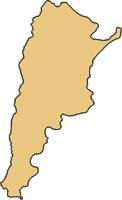
\includegraphics[width=0.6cm,height=1.2cm]{Imagenes/argentina.jpg}\\
\hline
2 & Brasil & 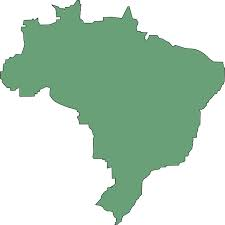
\includegraphics[width=1.5cm,height=1.5cm]{Imagenes/brasil.jpg}\\
\hline
\end{tabular}\\
\end{center}
\ \\
Y adem\'as brindar herramientas que permitan comparar eficientemente datos como los de la tercer columna.

\subsection*{Bases de Datos Espaciales}
\textbf{Definici\'on 1:} Es una Base de Datos que es optimizada para almacenar y consultar informaci\'on relacionada a objetos en el espacio, incluyendo puntos, l\'ineas y pol\'igonos.\\
\textbf{Definici\'on 2:} Es una colecci\'on de datos espaciales y no espaciales que est\'an interrelacionados.\\
\ \\
Deben permitir la descripci\'on de los objetos espaciales mediante tres caracter\'isticas:\\
\ \\
\begin{itemize}
\item \textbf{Atributos}: qu\'e es un objeto de acuerdo a sus caracter\'isticas.
\item \textbf{Localizaci\'on}: conocer d\'onde est\'a el objeto y qu\'e lugar ocupa.
\item \textbf{Topolog\'ia}: mejorar la interpretaci\'on sem\'antica del contexto y establecer jerarqu\'ias.
\end{itemize}

\subsubsection*{DBMS Espacial}
\begin{itemize}
\item \textit{Un SDBMS es un DBMS.}
\item \textit{Ofrece datos espaciales (SDTs) en su modelo de datos y su lenguaje de consulta.}
\item \textit{Soporta tipos de datos espaciales en su implementaci\'on, proveyendo al menos indexaci\'on espacial y algoritmos eficientes para joins espaciales.}
\end{itemize}
Un \textit{SDBMS} es un \textit{DBMS}. Suena trivial; refleja el hecho de que la informaci\'on espacial o geom\'etrica est\'a, en pr\'actica, conectada con la informaci\'on \textit{no-espacial}. El \textit{SDBMS} tiene propiedades adicionales para manejar datos espaciales.\\
\ \\
\textbf{Tipos de datos espaciales:} POINT, LINE, REGION, etc\'etera.\\
Proveen una abstracci\'on fundamental para modelar la estructura de entidades geom\'etricas en el espacio, as\'i como sus relaciones, propiedades y operaciones.
\subsubsection*{Objetivos de un SDBMS}
Deben integrar la representaci\'on y manipulaci\'on de datos geom\'etricos y espaciales con los datos no espaciales en un nivel l\'ogico y adem\'as proveer un soporte eficiente para almacenar y procesar datos a nivel f\'isico.
\subsubsection*{Requerimientos de un SDBMS}
\begin{itemize}
\item El lenguaje de consulta debe incorporar nuevas funciones sobre componentes geom\'etricos.
\item Utilizar m\'etodos de acceso eficientes.
\item Incorporar nuevos algoritmos para procesar consultas que satisfacen combinaciones de restricciones.
\item La representaci\'on l\'ogica debe ser extendida a datos geom\'etricos.
\item Capacidad de manejar grandes colecciones de objetos geom\'etricos.
\end{itemize}
\subsection*{Hacia un modelo de datos espacial}
Asumiendo aplicaciones 2-d y GIS, existen dos aspectos importantes que necesitan ser representados:\\
\begin{itemize}
\item \textbf{Objetos en el Espacio}: distinguir entre entidades espaciales de acuerdo a su representaci\'on geom\'etrica.
\item \textbf{Espacio}: describir cada punto del espacio, es decir, tener una idea de la representaci\'on del espacio mismo.
\end{itemize}
\subsubsection*{Modelando Datos Espaciales}
Los datos espaciales tienen las siguientes desventajas:
\begin{itemize}
\item Estructura compleja.
\item Las SBD tienden a ser muy grandes.
\item No existe un \'algebra est\'andar.
\item Operadores no cerrados.
\item Costo computacional elevado.
\end{itemize}
Es por ello que hay que implementar algoritmos y estructuras de datos que optimicen la manipulaci\'on de los mismos.
\subsubsection*{Objetos en el Espacio}
Son objetos \'unicos e individuales. Para modelarlos, las abstracciones fundamentales son el \textit{punto}, la \textit{l\'inea} y la \textit{regi\'on} (pol\'igono).\\
\ \\
\begin{center}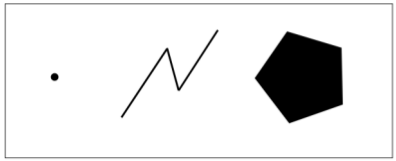
\includegraphics[width=8cm,height=3cm]{Imagenes/figurasgeom.png}
\end{center}
\subsubsection*{Punto}
Un punto representa el aspecto geom\'etrico de un objeto para el cual lo \'unico relevante es su localizaci\'on en el espacio.
Por ejemplo, una ciudad puede ser modelada como un punto en un mapa.\\
\ \\
\begin{center}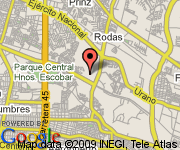
\includegraphics[width=3cm,height=3cm]{Imagenes/mapa1.png}
\end{center}
\subsubsection*{L\'inea}
Una l\'inea representa es la abstracci\'on b\'asica del movimiento a trav\'es del espacio, o conexiones en espacio.
Por ejemplo, r\'ios, carreteras, cables de tel\'efono, etc\'etera.\\
Usualmente representadas como \textit{polil\'ineas}, i.e, secuencias de segmentos.
\subsubsection*{Regi\'on o pol\'igono}
Una regi\'on es una abstracci\'on para algo que tenga una extensi\'on en el espacio 2-d. Por ejemplo un pa\'is, un lago, un parque nacional, etc\'etera. Una regi\'on puede tener huecos y puede ser conformada por distintos objetos del espacio.\\
\ \\
\begin{center}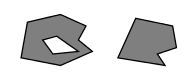
\includegraphics[width=4cm,height=1.8cm]{Imagenes/poligonos.png}
\end{center}
\subsubsection*{Espacio}
Hay que caracterizar los puntos del espacio. De esta forma, podemos modelar mapas tem\'aticos que indiquen por ejemplo, la divisi\'on de un pa\'is en provincias. Existen dos importantes instancias en las colecciones de objetos relacionadas espacialmente (espacio):son las \textit{particiones} y las \textit{redes}.
\subsubsection*{Particiones}
Una \textit{partici\'on} puede ser vista como un conjunto de regiones que son disjuntas. La adyacencia en este caso tiene un inter\'es particular; pares de regiones que tienen frontera com\'un. Pueden ser usadas para representar mapas.
\ \\
\begin{center}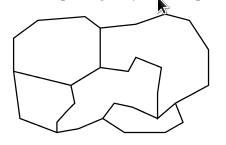
\includegraphics[width=3cm,height=1.8cm]{Imagenes/particion.png}
\end{center}
\subsubsection*{Redes}
Una red puede ser vista como un grafo embebido en el plano. Est\'a compuesta por un conjunto de objetos puntos (nodos) y un conjunto de objetos l\'ineas (aristas). Pueden ser usadas para representar elementos geogr\'aficos como carreteras, r\'ios, transportes p\'ublicos, etc\'etera.
\ \\
\begin{center}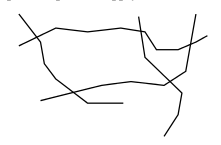
\includegraphics[width=3cm,height=1.8cm]{Imagenes/red.png}
\end{center}

\subsubsection*{Otras abstracciones}
Hemos mencionado hasta aqu\'i las m\'as comunes. Obviamente, existen otras como las \textit{particiones anidadas} (e.g. un pa\'is divido en provincias, y a su vez cada provincia en estados), o los modelos de terrenos digitales, para representar relieves.\\
\ \\
\begin{center}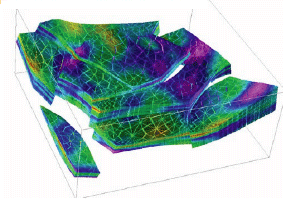
\includegraphics[width=3cm,height=2.5cm]{Imagenes/relieves.png}
\end{center}

\subsubsection*{Organizando el Espacio}
La geometr\'ia Euclidiana no es adecuada como una base para modelar en las bases de datos espaciales.
\begin{itemize}
\begin{small}
\item El espacio Eucl\'ideo es \textbf{cont\'inuo}, i.e., los puntos son representados como un par de n\'umeros reales: $p = (x,y) \in \mathbf{R}^{2}$.
\item Pero la computadora trabaja en forma \textbf{discreta}.
\begin{itemize}
\item $\Rightarrow$ el espacio es representado por un \textit{raster discreto}.
\end{itemize}
\end{small}
\end{itemize}
\textbf{Ejemplo:} Intersecci\'on de dos l\'ineas
\begin{itemize}
\begin{small}
\item El punto de intersecci\'on es redondeado al punto de la grilla m\'as cercano.
\item Una prueba para determinar si el punto de intersecci\'on est\'a en una de las l\'ineas determina un resultado falso.
\end{small}
\end{itemize}
\begin{center}
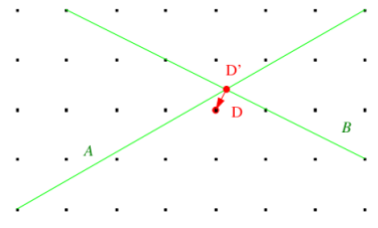
\includegraphics[width=4cm,height=3cm]{Imagenes/1.png}
\end{center}
\textbf{Soluci\'on:} Definir una base geom\'etrica discreta para modelar el espacio, as\'i tambi\'en como para lidiar con su implementaci\'on.\\
\ \\
Dos intentos para una base geom\'etrica:
\begin{itemize}
\item \textbf{Simplicial complexes} (Frank \& Kuhn)
\item \textbf{Realms} (G\"uting \& Schneider)
\end{itemize}

\subsubsection*{Organizando el Espacio: Simplicial Complexes}
Conceptos b\'asicos de \textbf{simplicial complexes}
\begin{itemize}
\item \textbf{d-simplex}: Un objeto de dimensi\'on d (ver Figura 4.5).
\begin{figure}[h]\center
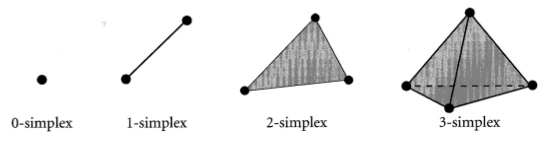
\includegraphics[width=6cm,height=2cm]{Imagenes/2.png}
\caption{Simplices de diferentes dimensiones}\end{figure}
\item \textbf{Simplicial Complex:} Un conjunto finito de simplices tales que la intersecci\'on de dos simplices cualquiera en el conjunto es un componente usado en los simplices (ver Figura 4.6).
\begin{figure}[h]\center 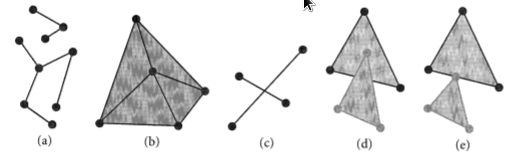
\includegraphics[width=6cm,height=2cm]{Imagenes/3.png} \caption{Intersecci\'on de simplices formando componentes}\end{figure}
\end{itemize}

\subsubsection*{Organizando el Espacio: Realm}
\textbf{Realm:} Un conjunto finito de puntos y segmentos de l\'ineas definidos sobre una grilla tal que:
\begin{small}
\begin{itemize}
\item cada punto o punto final de los segmentos es un punto en la grilla
\item cada punto final de un segmento es un punto del realm
\item ning\'un punto del realm se encuentra dentro de un segmento
\item dos segmentos no se intersecan salvo en sus puntos finales
\end{itemize}
\end{small}
Realm provee una descripci\'on completa de la geometr\'ia (puntos y l\'ineas), como puede observarse en la siguiente figura:
\begin{center}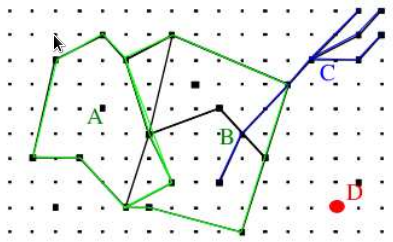
\includegraphics[scale=0.3]{Imagenes/4.png}\end{center}
\begin{small}
\end{small}

\subsubsection*{Tipos de Datos y \'Algebras Espaciales}
Las b\'asicas abstracciones espaciales pueden ser embebidas en un DBMS existente usando tipos abstractos de datos.
\begin{itemize}
\item \textbf{Tipos de Datos Espaciales} encapsulan
\begin{itemize}
\item la estructura de un objeto espacial, e.g., regi\'on
\item operaciones sobre esas estructuras
\end{itemize}
\item \textbf{\'Algebra Espacial}, es una colecci\'on de datos espaciales con operaciones relacionadas
\begin{itemize}
\item Completitud y clausura deben ser propiedades del \'algebra
\end{itemize}
\end{itemize}

\subsubsection*{\'Algebra ROSE}
El \'algebra de ROSE (RObust Spatial Extension, G\"uting \& Schneider) es un \'algebra espacial con tipos de datos espaciales basados en el modelo Realm (esto es, objetos compuestos por elementos Realm).
Este \'algebra utiliza como tipos de datos puntos, l\'ineas y regiones.\\
\begin{figure}[h]
\caption{Tipos de datos del \'algebra de ROSE}
\begin{center}
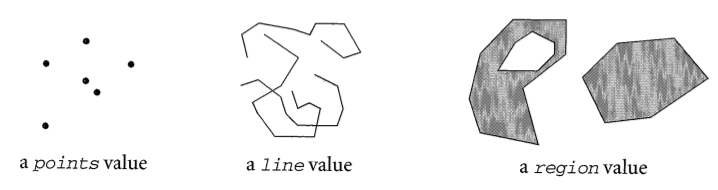
\includegraphics[scale=0.4]{Imagenes/5.png}
\end{center}
\end{figure}

\subsubsection*{\'Algebra ROSE: Operaciones}
Teniendo en cuenta los siguientes conjuntos:\\EXT = $\lbrace$l\'ineas, regiones$\rbrace$\ \ \ \ GEO = $\lbrace$puntos, l\'ineas, regiones$\rbrace$\\podemos definir las operaciones sobre el \'algebra de ROSE de la siguiente manera:
\begin{itemize}
\item Predicados espaciales para relaciones topol\'ogicas:
\begin{itemize}
\item \textbf{inside}: geo $\times$ regions $\rightarrow$ bool
\item \textbf{intersect, meets}: ext1 $\times$ ext2 $\rightarrow$ bool
\item \textbf{adjacent, encloses}: regions $\times$ regions $\rightarrow$ bool
\end{itemize}
\item Operaciones que devuelven tipos de datos espaciales at\'omicos:
\begin{itemize}
\item \textbf{intersection}: lines $\times$ lines $\rightarrow$ points
\item \textbf{intersection}: regions $\times$ regions $\rightarrow$ regions
\item \textbf{plus, minus}: geo $\times$ geo $\rightarrow$ geo
\item \textbf{contour}: regions $\rightarrow$ lines
\end{itemize}
\end{itemize}
\begin{itemize}
\item Operadores espaciales que devuelven n\'umeros:
\begin{itemize}
\item \textbf{dist}: geo1 $\times$ geo2 $\rightarrow$ real
\item \textbf{perimeter, area}: regions $\rightarrow$ real
\end{itemize}
\item Operadores espaciales en conjuntos de objetos:
\begin{itemize}
\item \textbf{sum}: set(obj) $\times$ (obj $\rightarrow$ geo) $\rightarrow$ geo
\item Alguna funci\'on espacial agregada como por ejemplo la suma de las \'areas de las provincias determinan el \'area de un pa\'is.
\item \textbf{closest}: set(obj) $\times$ (obj $\rightarrow$ geo1) $\times$ geo2 $\rightarrow$ set(obj)
\item Determina dentro de un conjunto de objetos aquellos cuyo atributo espacial tiene m\'inima distancia.
\item Otras operaciones complejas...
\end{itemize}
\end{itemize}

\subsubsection*{\'Algebra ROSE: Propiedades}
Estos ejemplos son suficientes para ver qu\'e tipo de operaciones est\'an disponibles en un \'algebra espacial.\\
Algunas propiedades que debe tener el \'algebra espacial son:
\begin{itemize}
\item Extensibilidad
\item Completitud
\item ?`Uno o m\'as tipos?
\item Operaciones de conjuntos
\end{itemize}

\subsubsection*{Relaciones Espaciales}
Entre las operaciones espaciales, podemos distinguir las \textit{relaciones}.
\begin{itemize}
\item Topol\'ogicas: adjacent, inside, disjoint. Son invariantes dentro de transformaciones topol\'ogicas como scaling, rotation, translation.
\item De direcci\'on: above, below, north\_of.
\item M\'etricas: distance $<$ 100.
\end{itemize}
Seis relaciones topol\'ogicas v\'alidas entre dos regiones simples (sin huecos, conectadas): \textit{disjoint, in, touch, equal, cover, overlap}.

\subsubsection*{Integrando la Geometr\'ia en el Modelo de Datos}
Los tipos de datos espaciales pueden ser embebidos en cualquier modelo de datos, e.g., el modelo relacional. El modelo de datos del DBMS debe ser extendido al nivel de tipos de datos at\'omicos, como strings y enteros.
La idea b\'asica es representar \textbf{objetos espaciales} con objetos (del modelo de datos del DBMS) con al menos un atributo espacial.\\
Los objetos espaciales son tuplas con al menos un atributo espacial.\\
\ \\
\texttt{\textbf{relation} estados (ename: STRING; area:REGION; epop: INTEGER)}\\
\texttt{\textbf{relation} ciudades (cname: STRING; centro:POINT; ext:REGION; cpop: INTEGER)}\\
\texttt{\textbf{relation} rios (rname: STRING; ruta:LINE)}

\subsubsection*{Consultas}
Dos problemas principales:
\begin{itemize}
\item Conectar las operaciones del \'algebra espacial (incluyendo los predicados de relaciones espaciales) a las facilidades de un lenguaje de consulta de un DBMS.\\
Los operadores fundamentales son:
\begin{itemize}
\item Spatial selection
\item Spatial join
\item Overlay, fusion, ...
\end{itemize}
\item Proveer una representaci\'on gr\'afica de la informaci\'on espacial (o sea, los resultados de la consulta) y adem\'as una entrada gr\'afica para los valores en las consultas.
\end{itemize}

\subsubsection*{Consultas: Selecci\'on Espacial}
\textbf{Selecci\'on Espacial}: retorna aquellos objetos que satisfacen un predicado espacial en la consulta.\\
\ \\
\textit{Todas las ciudades de Argentina}\\
\texttt{SELECT cname FROM ciudades c \\
WHERE c.centro inside Argentina.area}\\
\ \\
\textit{Todas las grandes ciudades en un radio de 100km de Rosario}\\
\texttt{SELECT cname FROM ciudades c \\
WHERE dist(c.centro, Rosario.centro) < 100\\
\ \ \ AND c.pop > 500k}

\subsubsection*{Consultas: Join Espacial}
\textbf{Join Espacial:} un join que compara cualesquiera dos objetos que fueron \textit{joineados} basado en un predicado que toma los valores espaciales de ambos.\\
\ \\
\textit{Para cada r\'io de Argentina, encontrar todas las ciudades dentro de 50 kms}\\
\texttt{SELECT r.rname, c.cname, length(intersection(r.ruta, c.area))\\
FROM rios r, ciudades c \\
WHERE r.ruta intersects Argentina.area \\
\ \ \ AND dist(r.ruta, c.area) < 50}

\subsubsection*{Consultas: Otras operaciones}

\textbf{Overlay:} retorna las regiones que son el resultado de sobreposicionar dos particiones.\\
\textbf{Fusion:} es una forma especial de agrupaci\'on. Para cada grupo obtenido, se forma la uni\'on de todos los valores de un atributo espacial.\\
\textbf{Voronoi:} computa de una colecci\'on de objetos puntos \textit{S} la correspondiente colecci\'on de objetos regi\'on. Para cada punto \textit{p}, la regi\'on consiste de los puntos del plano m\'as cercanos a \textit{p}, y que no est\'en m\'as cercanos a otro punto de \textit{S}.  


\subsubsection*{Consultas: I/O Gr\'afica}
?`C\'omo determinar \texttt{Argentina} en los ejemplos anteriores(input), o c\'omo mostrar \texttt{intersection(ruta,Argentina.area)} o \texttt{rio.ruta}(output)?\\
\ \\
Requerimientos para consultas espaciales:
\begin{itemize}
\item Tipos de datos espaciales.
\item Muestreo gr\'afico de los resultados de consulta.
\item Combinaci\'on gr\'afica de varios resultados de consultas.
\item Herramientas para interactuar con gr\'aficos de entrada y resultados.
\item Facilidad para verificar el contenido de una muestra.
\end{itemize}

\subsubsection*{Formato de Datos Espaciales}
Existen dos est\'andares de representaci\'on:
\begin{itemize}
\item \textbf{WKT} (Well Known Text)
\item \textbf{WKB} (Well Known Binary)
\end{itemize}

\subsubsection*{Formato de Datos Espaciales: WKT}
Esta representaci\'on es una codificaci\'on en formato ASCII para describir objetos espaciales. Es usada por \textit{PostgreSQL} en \textit{PostGIS}, y tambi\'en en Google Maps. Podemos describir puntos, multipuntos, l\'ineas, pol\'igonos, multipol\'igonos, puntos en 3 dimensiones, etc\'etera.\\
\ \\
Sintaxis:
\begin{itemize}
\item Punto: \texttt{POINT(30 50)}
\item L\'inea: \texttt{LINESTRING(1 1, 5 5, 10 10)}
\item Pol\'igono: \texttt{POLYGON ( (0 0, 10 0, 10 10, 0 10, 0 0),(20 20, 20 40, 40 40, 40 20, 20 20))}
\end{itemize}

\subsubsection*{Formato de Datos Espaciales: WKB}
WKB utiliza enteros sin signo de un byte, enteros sin signo de cuatro bytes, y n\'umeros de ocho bytes de doble precisi\'on (formato IEEE 754). Un byte son ocho bits. Por ejemplo, un valor WKB que corresponde a un \texttt{POINT(1 1)} consiste en esta secuencia de 21 bytes (cada uno representado aquí por dos d\'igitos hexadecimales):\\
\texttt{0101000000000000000000F03F000000000000F03F}\\
\ \\
\begin{tabular}{l l}
Orden de byte & 01 $\rightarrow$ LE o BE\\
Tipo WKB	  & 01000000 $\rightarrow$ tipo de objeto\\
X & 000000000000F03F\\
Y & 000000000000F03F\\
\end{tabular}\\
\ \\
M\'as r\'apida que WKT, pero menos entendible para el usuario.

\subsection*{Indexaci\'on Espacial}

Organiza el espacio y los objetos en \'el de forma tal que s\'olo son considerados la parte del espacio y los objetos que sean relevantes a una consulta. B\'asicamente, es un mecanismo para decrementar el n\'umero de b\'usquedas. El objetivo principal es tratar de no visitar y tocar cada vez a todos los \textit{n} elementos en la BD. Los \'indices espaciales nos permiten optimizar la recuperaci\'on.\\

\begin{figure}[h]
\center
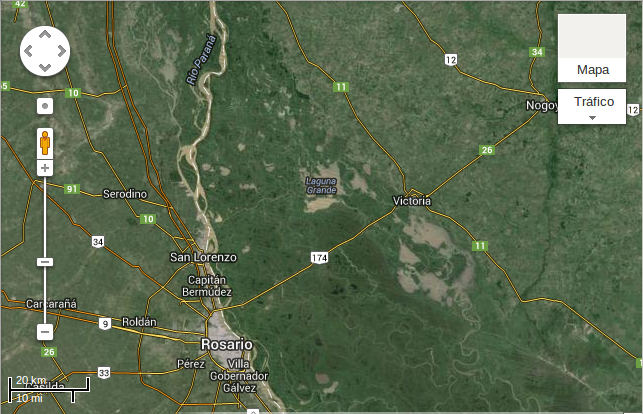
\includegraphics[scale=0.5]{Imagenes/6.png}
\caption{Im\'agen de Google Maps donde se utilizan m\'etodos de indexaci\'on espacial}
\end{figure}
\noindent El uso principal de la indexaci\'on es para la selecci\'on espacial, pero es usado tambi\'en para otras operaciones como join espacial o encontrar el objeto m\'as cercano.\\
Dos enfoques principales de la indexaci\'on espacial:
\begin{itemize}
\item Mapear objetos espaciales al espacio 1-D y utilizar t\'ecnicas est\'andar de indexaci\'on, como B-trees
\item Estructuras de indexaci\'on espacial dedicadas, como R-trees
\end{itemize}

\subsubsection*{Indexaci\'on Espacial: R-Tree}
\textbf{R-Tree} es una estructura de datos similar a los \textit{B-Trees}, con la diferencia que se utilizan para m\'etodos de acceso espacial. Es decir, podemos indexar coordenadas por ejemplo.\\
Cada nodo tiene un n\'umero variable de entradas, y cada entrada almacena dos datos: una forma de identificar a un nodo hijo y el conjunto l\'imite de todas las entradas de ese nodo hijo.\\
\textbf{B\'usqueda:} recursiva desde la ra\'iz, se verifica si el rect\'angulo de la consulta se solapa con alg\'un rect\'angulo del nodo.\\
\textbf{Inserci\'on:} partiendo de la ra\'iz, se usa una heur\'istica para seleccionar el nodo candidato.
\begin{figure}[h]
\begin{center}
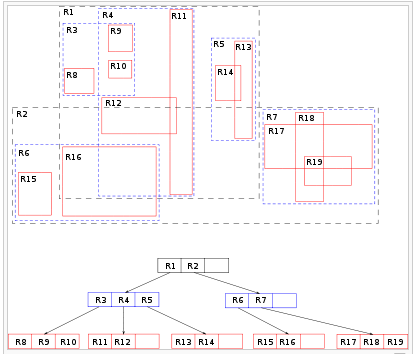
\includegraphics[scale=0.5]{Imagenes/20.png}
\end{center}
\caption{Estructura del R-Tree}
\end{figure}

\noindent La idea fundamental de la indexaci\'on espacial es la aproximaci\'on.
\begin{itemize}
\item Aproximaci\'on continua
\item Aproximaci\'on por grilla
\end{itemize}
\begin{figure}[h]
\begin{center}
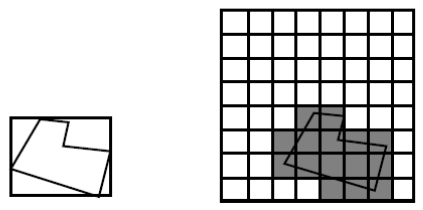
\includegraphics[scale=0.2]{Imagenes/7.png}
\caption{Aproximaci\'on continua a la izquierda, aproximaci\'on por grilla a la derecha}
\end{center}
\end{figure}
Para procesar una consulta, se procede a la estrategia de \textbf{filtrado y refinamiento}.
\begin{enumerate}
\item Filtrado: retorna un conjunto (donde est\'a la soluci\'on) de los valores posibles que satisfacen un predicado
\item Refinado: Para cada candidato, se refina la b\'usqueda chequeando la geometr\'ia
\end{enumerate}

\noindent Las estructuras espaciales son dise\~nadas para almacenar puntos (para objetos puntos) o rect\'angulos (l\'ineas y regiones). Las operaciones sobre esas estructuras son inserci\'on, borrado y pertenencia.\\
Consultas t\'ipicas:
\begin{itemize}
\item Puntos
\begin{itemize}
\item Consulta de rango: todos los puntos dentro de un rect\'angulo
\item Vecino m\'as cercano: el punto m\'as cercano a un punto consultado
\item Distancia: desde un punto, enumerar los puntos que est\'an a cierta distancia 
\end{itemize}
\item Rect\'angulos
\begin{itemize}
\item Intersecci\'on
\item Contenido
\end{itemize}
\end{itemize}


\subsubsection*{Indexaci\'on Espacial: Estructuras}
\begin{itemize}
\item Una estructura de indexaci\'on espacial dedicada organiza los objetos en \textbf{cubetas}.
\item Cada cubeta tiene asociada una \textbf{regi\'on}, que es, una parte del espacio que contiene todos los objetos almacenados en esa cubeta.
\item Para estructuras de datos de puntos, las regiones son disjuntas
\begin{itemize}
\item el espacio es particionado y cada punto pertenece a solo una partici\'on (cubeta)
\begin{center}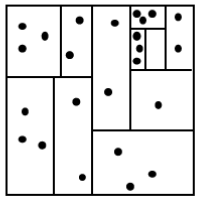
\includegraphics[scale=0.3]{Imagenes/8.png}
\end{center}\end{itemize}
\item Para estructuras con rect\'angulos, las cubetas pueden solaparse
\end{itemize}


\subsubsection*{Indexaci\'on Espacial: Estructura de Puntos}
Estructuras espaciales para puntos: en $k$ dimensiones son representadas como una tupla $t = (x_1,...,x_k)$\\
\ \\
\textbf{\'Indice de Grilla}: Estructura de indexaci\'on espacial para puntos (Nievergelt, Hinterberger y Sevcik 84)
\begin{center}
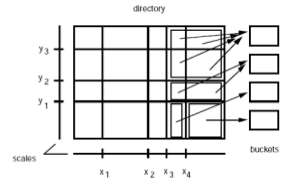
\includegraphics[scale=0.4]{Imagenes/9.png}
\end{center}

\begin{itemize}
\item El directorio es un arreglo $k$-dimensional cuyas entradas son punteros a las cubetas.
\item Todos los puntos en las celdas son almacenados en cubetas apuntando a la entrada de directorio correspondiente.
%\item Escalas peque\~nas. El directorio es almacenado en disco.
\end{itemize} 
\noindent \textbf{kd-tree:}\\
\'Arbol binario donde cada nodo interno contiene un valor clave de una dimensi\'on. La clave en el nodo ra\'iz (nivel 0) divide el espacio de datos con respecto a la dimensi\'on 0, las claves en sus hijos (nivel 1) divide los dos subespacios y as\'i sucesivamente hasta que se terminan las dimensiones, luego se reinicia el ciclo.\\
\begin{center}
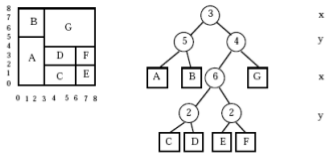
\includegraphics[scale=0.5]{Imagenes/10.png}
\end{center}

\noindent \textbf{quad-tree:}\\
Divide el espacio de datos en forma recursiva en 4 cuadrantes (NO, NE, SO, SE)\\
\begin{center} 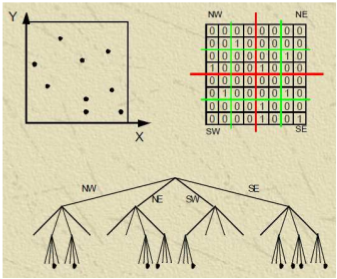
\includegraphics[scale=0.5]{Imagenes/11.png} \end{center}

\noindent \textbf{quad-tree:}\\
Hay diferentes algoritmos para procesar puntos, l\'ineas, pol\'igonos (i.e., distintos tipos de nodos, algoritmos de consultas).
Es usado muy frecuentemente en GIS comerciales para comprimir, almacenar y manipular im\'agenes raster.\\
\begin{center} 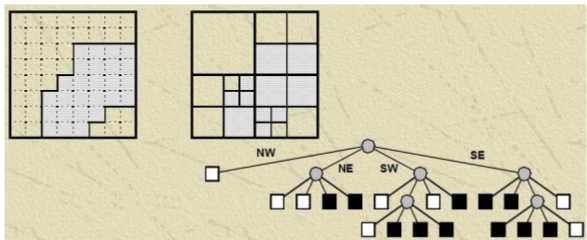
\includegraphics[scale=0.5]{Imagenes/12.png} \end{center}

\subsubsection*{Indexaci\'on Espacial: Estructura de Rect\'angulo}
Dos enfoques principales:
\begin{itemize}
\item Solapamiento de regiones
\item Clipping (Recorte)
\end{itemize}

\subsubsection*{Indexaci\'on Espacial: Estructura de Rect\'angulo}
\textbf{Solapamiento de regiones:} se abandona el espacio particionado y las regiones pueden solaparse, e.g., \textbf{R-tree}.
\begin{itemize}
\item Ventaja: El objeto espacial (clave) est\'a en una sola cubeta.
\item Desventaja: Muchos caminos terminan en un solapamiento de cubetas.
\end{itemize}
\begin{center}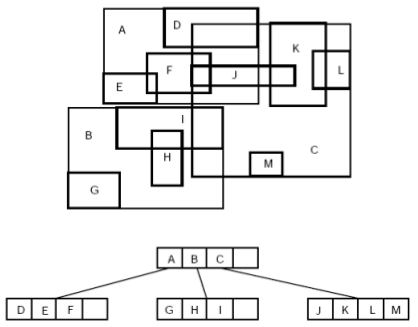
\includegraphics[scale=0.3]{Imagenes/13.png}
\end{center}

\noindent \textbf{Recorte (Clipping):} las cubetas son disjuntas, pero los rect\'angulos son cortados en varias piezas, e.g., \textbf{R$^+$-tree}.
\begin{itemize}
\item Ventaja: Menos ramas en el \'arbol
\item Desventaja: M\'ultiples entradas para un objeto espacial
\end{itemize}
\begin{center}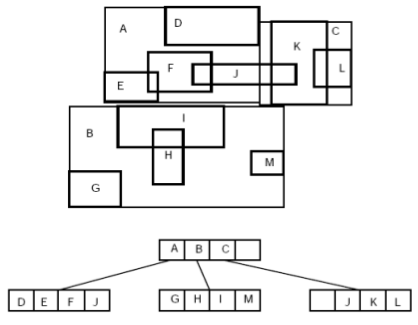
\includegraphics[scale=0.5]{Imagenes/14.png}
\end{center}

\subsection*{Estado del Arte: Las BDE en la actualidad}

\subsubsection*{Spatial SQL}

\textit{SQL espacial} brinda soporte para nuevos tipos de datos como:
\begin{itemize}
\item Point
\item LineString
\item Polygon
\item MultiPoint
\item etc\'etera...
\end{itemize}
Relaciones entre objetos:
\begin{itemize}
\item ST\_Contains
\item ST\_Equals
\item ST\_Intersects
\item ST\_Touches
\item etc\'etera...
\end{itemize}
Constructores de objetos:
\begin{itemize}
\item ST\_MultiLineString
\item ST\_Point
\item ST\_MultiPolygon
\item ST\_MultiCurve
\item etc\'etera...
\end{itemize}
\subsubsection*{Spatial SQL: Ejemplo}
Crear una tabla nueva:\\
\ \\
\texttt{CREATE TABLE Rio(\\
\ \ \ \ \ Nombre varchar(30),\\
\ \ \ \ \ Origen varchar(30),\\
\ \ \ \ \ Longitud number,\\
\ \ \ \ \ Forma LineString );}\\
\ \\
\textbf{Consulta:} encontrar nombres de pa\'ises que son vecinos de Estados Unidos en la tabla Pa\'ises.\\
\ \\
\texttt{SELECT P1.Nombre\\
FROM Paises P1, Paises P2\\
WHERE Touch(P1.Forma,P2.Forma)=1\\
AND P2.Nombre = USA}\\
\ \\
\textbf{Consulta:} encontrar la distancia entre dos puntos, dada una tabla de puntos.\\
\ \\
\texttt{SELECT ST\_Distance(geometrycolumn,\\
\ \ \ \ ST\_GeomFromText('POINT(1 2)',4326)\\
FROM tabladepuntos\\
ORDER BY\\
ST\_Distance(geometrycolumn,\\
\ \ \ \ ST\_GeomFromText('POINT(1 2)',4326) LIMIT 10)}
\subsubsection*{Alternativas Espaciales}
Algunas de las elecciones que podemos hacer hoy en d\'ia en materia de DBMS espaciales son:\\
\ \\
\textbf{Open Source}
\begin{itemize}
\item MySql (actualmente viene con soporte espacial)
\item MongoDB (no relacional)
\item MariaDB
\item PostgreSQL $+$ PostGIS
\item SpatialDB
\item y m\'as ...
\end{itemize}
\textbf{Pagos}
\begin{itemize}
\item Oracle
\item SQL Server
\end{itemize}

\subsubsection*{PostgreSQL $+$ PostGIS}
\begin{center}
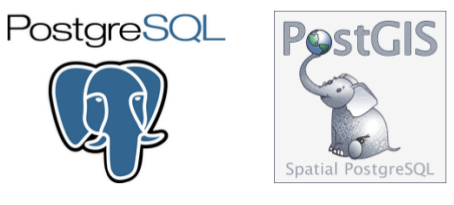
\includegraphics[scale=0.3]{Imagenes/23.png}
\end{center}
\textbf{PostgreSQL}\\
PostgreSQL es un sistema administrador
 de bases de datos objeto-relacional 
basado en POSTGRES, desarrollado en la Universidad de California 
en Berkeley, en el Departamento de Ciencias de la Computación. POSTGRES fue 
pionero de muchos conceptos que solo estuvieron disponibles en algunos 
sistemas de bases de datos comerciales mucho más tarde. 
PostgreSQL es un proyecto desarrollado
 con código abierto que soporta el 
estándar SQL y ofrece muchas características interesantes: 

\begin{itemize}
\item Consultas complejas
\item Claves for\'aneas
\item Disparadores
\item Vistas
\item Integridad transaccional
\item Control de concurrencia
\end{itemize}

Adem\'as PostgreSQL puede ser ampliado 
por el usuario de muchas formas,
mediante la adici\'on de nuevas definiciones de: 

\begin{itemize}
\item Tipos de datos
\item Funciones
\item Operadores
\item Funciones de agregado
\item M\'etodos indexados
\item Lenguajes procedurales
\end{itemize}

Debido a que es de licencia libre, PostgreSQL puede ser usado, modificado 
y distribuido por todo el mundo de forma gratuita para cualquier fin, ya sea privado, comercial o acad\'emico. Es considerado
 como uno de los mejores gestores de 
bases de datos de software libre. Muchas 
empresas han iniciado el uso de esta herramienta benefici\'andose en la reducci\'on de los costos y en el aumento de la fiabilidad.  

\textbf{PostGIS}
PostGIS es una extensi\'on del sistema de bases de datos objeto-relacional 
PostgreSQL, que permite el uso de objetos geogr\'aficos. Fue creado por 
Refractions Research Inc, como un proyecto de investigaci\'on de tecnolog\'ia de bases de datos espaciales.\\
\ \\
Geometr\'ias b\'asicas soportadas:

\begin{itemize}
\item POINT 	(x y)
\item LINESTRING (x$_1$ y$_1$, ...,x$_n$ y$_n$)
\item POLYGON (x$_1$ y$_1$, ...,x$_n$ y$_n$)
\end{itemize}

Tambi\'en brindan soporte para multi-geometr\'ias:

\begin{itemize}
\item MULTIPOINT ((POINT$_1$), ...,(POINT$_n$))
\item MULTILINESTRING ((LINESTRING$_1$), ...,(LINESTRING$_n$))
\item MULTIPOLYGON ((POLYGON$_1$), ...,(POLYGON$_n$))
\end{itemize}

Los constructores, operadores y relaciones son los que vienen con Spatial SQL, es decir, los mencionados anteriormente. \textit{PostGIS} agrega caracter\'isticas interesantes como su propio spatial join, GIS overlay functions, primitivas 2D y 3D, adem\'as de un entorno de desarrollo amigable.\\
\begin{figure}[h]
\begin{center}
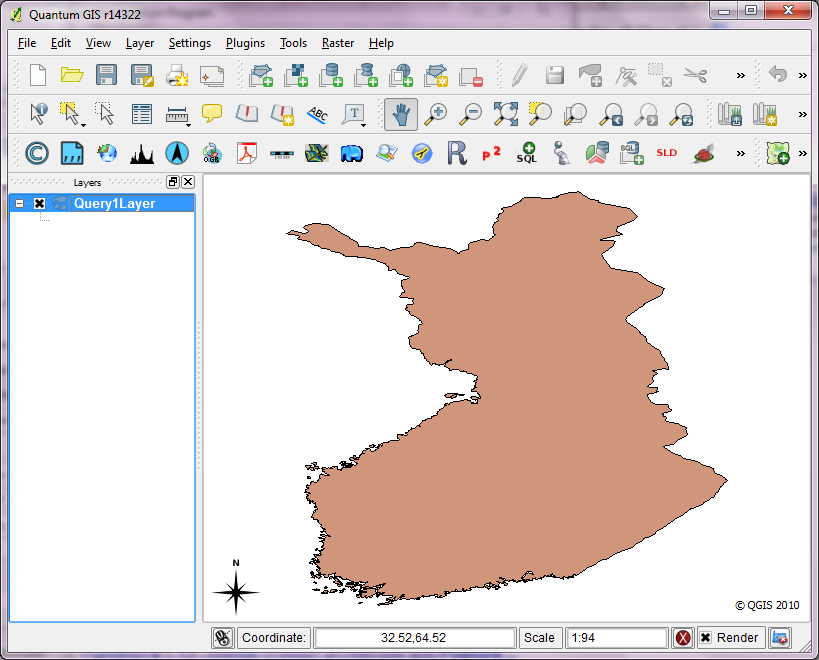
\includegraphics[scale=0.2]{Imagenes/24.png}
\end{center}
\caption{Entorno de desarrollo PostGIS}
\end{figure}



\mychapter{5}{Bases de Datos Espacio-Temporales}

\bibliography{ref.bib}
\end{document}